\documentclass[11pt,twocolumn]{report}
\usepackage{graphicx}
\usepackage{a4wide}
\usepackage[english]{babel}
\usepackage{amsfonts}
\usepackage{amsthm}
\usepackage{amsmath}
\graphicspath{ {images/} }

\author{He Chen, Henri Maxime Demoulin, Gabrielle De Micheli}
\title{CIS520 Final Project Report}

\begin{document}
\maketitle
\section*{Methods Accuracy Report}
    % Results for each method you tried (try to use checkpoints to get test set accuracy for each of your methods)
    First, let us explain some of the preprocessing steps that we have taken.
    For the word count preprocessing, we deleted all the English, French, and Spanish common stop words, words containing only one character (punctuation?), unicode words starting with $\backslash u$, and words that are http and rt links. All of these preprocessing steps were tested one by one to confirm that it indeed does increase the cross validation accuracy. 

	Another thing that we have done to try and see which words are good to delete in the preprocessing was iterating through all 10,000 of the word columns, and if deleting that column yielded significantly better cross validation accuracy (1.5 percent of better), then we deleted that column in the preprocessing step. However, that did not work and we ended up with more cross validation error (2-3 percent) than we started with.
    
    \subsection*{Generative Methods}
    \subsubsection{Naive Bayes}
    We start by using Naive Bayes only on the words. This method gave us around $80 \%$ testing accuracy on the words without preprocessing. If we do the preprocessing described above, the testing accuracy rises to $81.42\%$. In order for Naive Bayes to work, we got rid of all the words that do not appear in any tweets, since $fitncb()$ had issues dealing with words of probability $0$. In order to use a variation of the bag of word model, the words are set to 1 if they appear in a tweet and zero otherwise.
    We have also tried and tested $\log(w_i + 1)$ and $\sqrt(w)$, but doing that made the accuracy of Naive Bayes go bad $(22-35)$ percent error. So we concluded that the best way was simply checking if the word exists or doesn't exist (0 or 1). 
	From our experience, Naive Bayes is both extremely accurate and extremely fast when used on the word counts.   
   
    
    \subsection*{Discriminative Methods}
    \subsubsection{Linear Regression}
    We tried many variants of linear regression on the CNN features. We tried with L1 regularization, L2 regularization, and elastic net. However, even the best (L2) was barely at 67% test accuracy, and when combined with the bag of words Naive Bayes, netted 79-80% cross validation accuracy. Therefore, while we did try things with linear regression, we were not successful in making it good enough to actually use. 
    
     \subsubsection{Random Forest}
     "We tried random forest only on the words but we observed the following: with 20 trees, we had a cross validation error of 0.2167 and with 100 trees a cross validation error of 0.2116. We use the same preprocessing process that with Naive Bayes".(DELETE MAYBE)\\
     For 100 trees, the cross validation error is 0.0533. For 500 trees, we get cross validation error of 0.0520 and for 1000 trees, we get a cross validation error of 0.0509. For the last case, the cross validation accuracy is 0.7776.
    \subsubsection{SVM}
    
    If we use SVM with an RBF (Radial Basis Function) kernel function, we have a cross validation error of 0.3813. Without RBF, the cross validation error is 0.26. The linear kernel is twice as accurate as the RBF function. However, if we use RBF but this time without the word-count, we have a cross validation error of 0.3776, which is greater than the error obtained with the two previous combinations we tried. If we try to use SVM without the word-count and without RBF, the cross validation error is 0.2626. We also try SVM only on words, and notice that it performs better than KNN.
    
    \subsubsection*{Perceptron}
    TO DO
    \subsection*{Instance based Methods}
    \subsubsection{KNN}
    
    We use KNN on all four datasets and get a traning error (cross-validation) of 0.3556.
   
    \subsection*{Regularization Method}
    our own regularization method other that the standard $L_i$ penalty....
    TO DO
    \subsection*{Semi-supervised dimensionality reduction}
    \subsubsection*{PCA}
    We try using PCA on the \textit{image dataset}. First, we use PCA with all the PCs combined with SVM which gives a cross validation error of 0.0324. We do the same again but only with 1000 PCs. This gives an error of 0.1198. Moreover, using 570 PCs (corresponding to 50MB), we get a cross validation error of 0.1509.\\
    
    
   On the \textit{word dataset}, we also try using PCA with various numbers of PCs (all, 500 ...) and this time, combined with random forest. This gives a cross validation error of 0.0064. The test-accuracy is 0.7491.\\
    
    

\section *{Methods Analysis}
    % Analysis of your experiments. What worked and what didn’t work? Why not? What did you do to try to fix it? Simply saying “I tried XX and it didn’t work” is not enough.
TO DO
\section*{Visualization}
    % An interesting visualization of one of your models. For instance, find the words that most correlate with the outcome. 
    We consider the well-classified words and we want to find which words are the most important. In order to visualize this, we compute a word cloud. 
    
    \begin{center}
    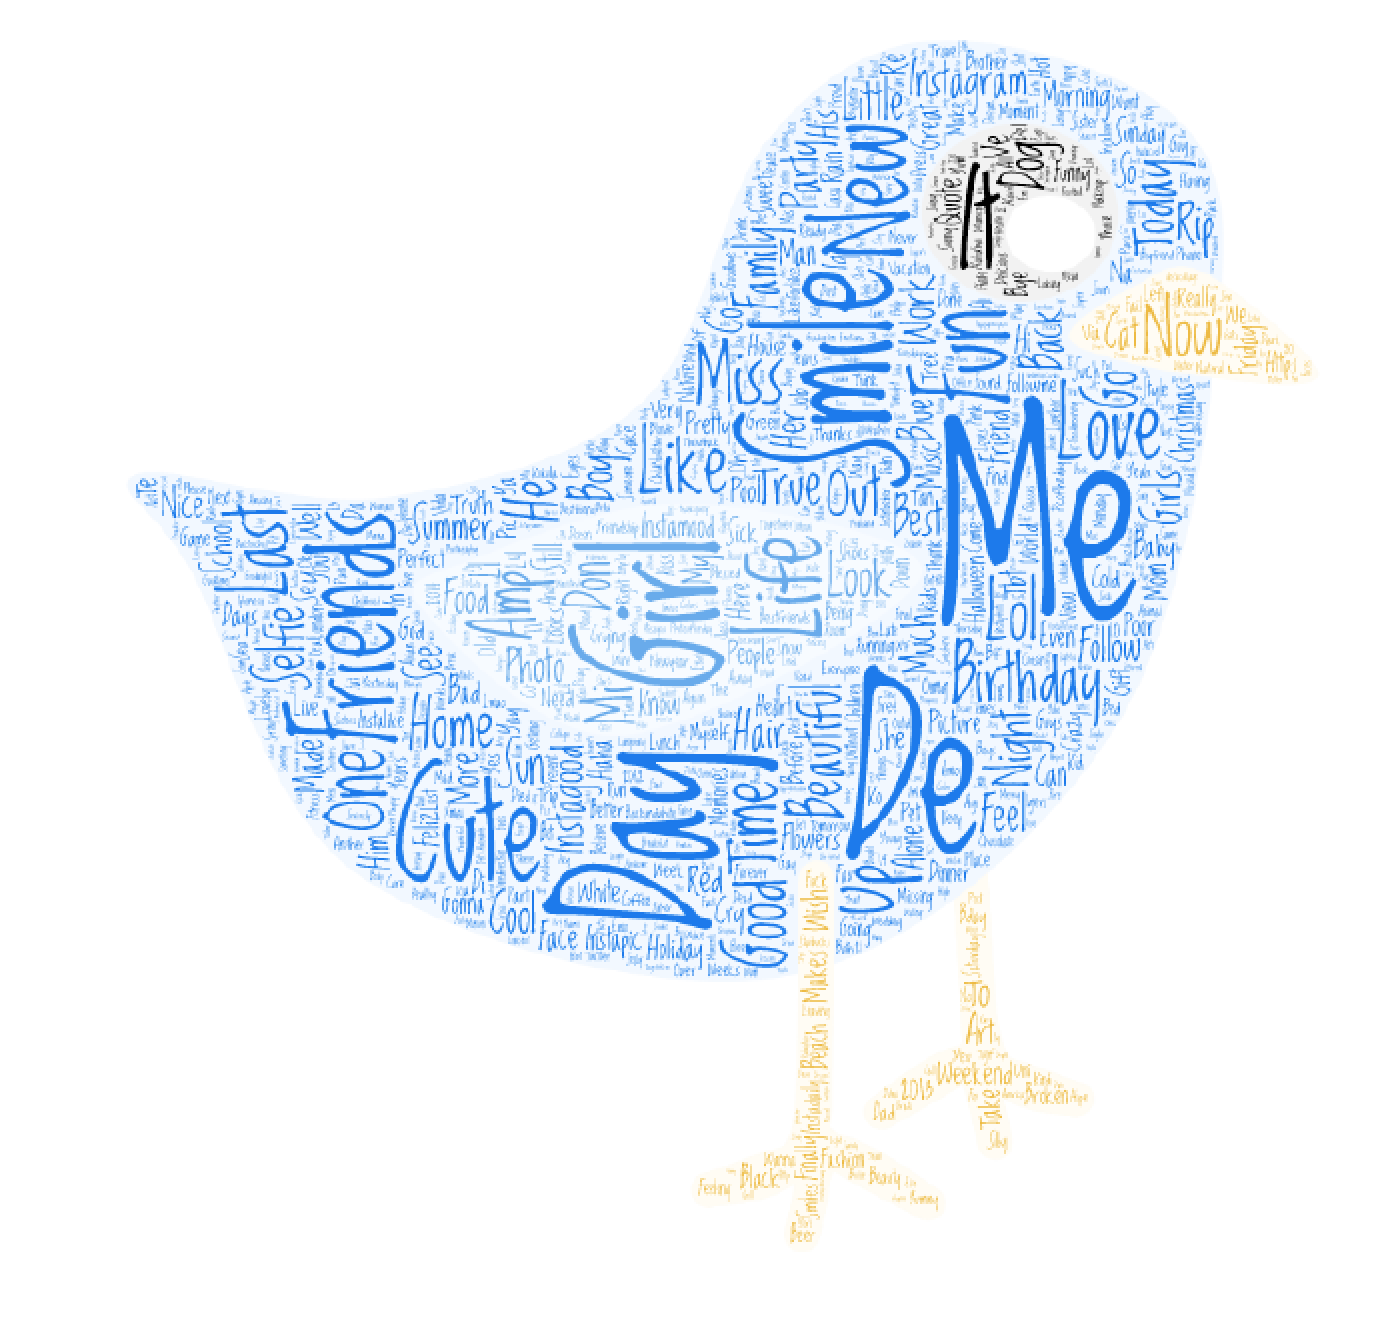
\includegraphics[scale=0.3]{cloud}
    \end{center}
    

\end{document}

